\documentclass[aspectratio=169,10pt]{beamer}
\usetheme{Madrid}
\usepackage{graphicx}
\usepackage{amssymb}

% Loại bỏ bóng đổ
\setbeamertemplate{blocks}[rounded][shadow=false]
\setbeamertemplate{navigation symbols}{}

% Color configuration
\definecolor{primaryblue}{RGB}{20, 55, 110}
\setbeamercolor{palette primary}{bg=primaryblue,fg=white}
\setbeamercolor{structure}{fg=primaryblue}

\begin{document}

\begin{frame}{Formal Definition: Function of Two Variables}
    \begin{columns}[T]
        % Cột trái: 2 Khung Definition và Boundary Convention
        \begin{column}{0.56\textwidth}
            \begin{block}{Definition (Function of Two Variables)}
                \small
                Let $z = f(x, y)$ be a function with two variables $x$ and $y$.
                \begin{itemize}
                    \item $x$ and $y$ are the \textbf{independent variables}.
                    \item $z$ is the \textbf{dependent variable}.
                    \item Unless otherwise specified, the \textbf{domain} $D$ is the \textbf{largest subset of $\mathbb{R}^2$} on which $f$ is mathematically well-defined.
                \end{itemize}
            \end{block}

            \vspace{0.1cm}

            \begin{block}{Boundary Convention for Domains in $\mathbb{R}^2$}
                \small
                \begin{itemize}
                    \item \textbf{Strict inequality ($>$ or $<$)}: Boundary drawn as a \textbf{dashed curve} (points excluded).
                    \item \textbf{Non-strict inequality ($\ge$ or $\le$)}: Boundary drawn as a \textbf{solid curve} (points included).
                \end{itemize}
            \end{block}
        \end{column}

        % Cột phải: Chứa Animation Manim minh họa trực quan
        \begin{column}{0.42\textwidth}
            \centering
            \vspace{0.1cm}
            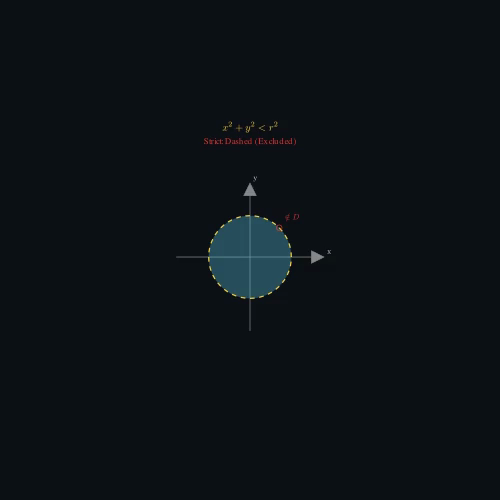
\includegraphics[width=0.88\linewidth, keepaspectratio]{DomainBoundaryScene.png}
            
            \vspace{0.1cm}
            {\tiny \textcolor{gray}{\textit{Dashed boundary vs. Solid boundary}}}
        \end{column}
    \end{columns}
\end{frame}

\end{document}
